% Copyright (c)  2010-2011  EDF-EADS.
% Permission is granted to copy, distribute and/or modify this document
% under the terms of the GNU Free Documentation License, Version 1.2
% or any later version published by the Free Software Foundation;
% with no Invariant Sections, no Front-Cover Texts, and no Back-Cover
% Texts.  A copy of the license is included in the section entitled "GNU
% Free Documentation License".




%%%%%%%%%%%%%%%%%%%%%%%%%%%%%%%%%%%%%%%%%%%%%%%%%%%%%%%%%%%%%%%%%%%%%%%%%%%%%%%%%%%%%%%%%% 
\section{Use Cases Guide}

This section presents the main functionalities of the module $otagrum$ in their context. As the module  $otagrum$ links the $openturns$ objects and the $pyagrum$ ones, we precise for each script from which library the python lines come from.\\
It is possible to have more exhaustive information on the $pyagrum$ module on the web site $http://agrum.lip6.fr$.



%%%%%%%%%%%%%%%%%%%%%%%%%%%%%%%%%%%%%%%%%%%%%%%%%%%%%%%%%%%%%%
\subsection{Which python modules to import ?}

In order to use the functionalities described in this documentation, it is necessary to import  : 
\begin{itemize}
   \item the $openturns$ python module which gives access to the Open TURNS functionalities,
   \item the $pyAgrum$ module which gives access to the aGrUM functionalities,
   \item the $otagrum$ module which links the $openturns$ functionalities and the $pyAgrum$ ones.
\end{itemize}

Python  script for this use case :

\begin{lstlisting}
# Load OpenTURNS to manipulate distributions
from openturns import *
# Load pyAgrum to define the Network
from pyAgrum import *
# Load the link between OT and aGrUM
from otagrum import *
\end{lstlisting}

%%%%%%%%%%%%%%%%%%%%%%%%%%%%%%%%%%%%%%%%%%%%%%%%%%%
\newpage \subsection{Creation of a Variable} \label{VariableCreation}

In $pyagrum$, it is possible to create three different kinds of discrete variables : 
\begin{itemize} 
  \item a categorial variable which labels are strings : the $LabelizedVar$,
  \item a discrete variable which range is a finite interval of $\mathbb{N}$ : the $RangeVar$,
  \item a discretized variable which is a real variable which range is discretized into a finite collection of intervals of $\mathbb{R}$ : $([T_0, T_1], \hdots, [T_{N-1}, T_N])$, where $T_O$ can be equal to $-\infty$ and
    $T_N$ equal to $+\infty$ : the $DiscretizedVar$.
\end{itemize}

%%%%%%%%%%%%%%%%%%%%%%%%%%%%%%%%%%%%%%%%%%%%%%%%%%%%%%%%%%%%%%
\subsubsection{UC : Creation of a Categorical Variable}

A categorical variable is a discrete variable which modalities are considered as labels. It may be some strings or even some numbers but considered as special strings.\\

This use case shows how to create such a variable : creation of the object and its modalities. The quantification step is described further in section \ref{BayesNetQuantification}.\\

The following lines are entirely part of the $pyagrum$ module. \\

\requirements{
  \begin{description}
  \item[$\bullet$] none
  \end{description}
}
{
  \begin{description}
  \item[$\bullet$] a Categorical variable  : {\itshape myCategoricalVar},
  \item[type:] a LabelizedVar
  \end{description}
}

\espace
Python  script for this use case :

\begin{lstlisting}
# Create a categorical variable

# Choose a name
name = 'light'
# Give a comment
comment = 'Intensity of the light'
# Fix the initial number of modalities to 0
initialNumberModalities = 0
myCategoricalVar = LabelizedVar(name, comment, initialNumberModalities)

# Add your labels : for example 3 labels
myCategoricalVar.addLabel("modality1")
myCategoricalVar.addLabel("modality2")
myCategoricalVar.addLabel("modality3")

# Print the created categorical variable
print myCategoricalVar

# Explicitate the label number i
# Care : numerotation begins at 0
print myCategoricalVar.label(2)

# Explicitate all the labels
print myCategoricalVar.labels()

# Erase all the declared labels 
# the categorical variable has no label any more
myCategoricalVar.eraseLabels()
\end{lstlisting}



%%%%%%%%%%%%%%%%%%%%%%%%%%%%%%%%%%%%%%%%%%%%%%%%%%%%%%%%%%%%%%
\newpage \subsubsection{UC : Creation of a Discrete Variable }

The considered discrete variables have a finite interval of $\mathbb{N}$ as range. \\

This use case shows how to create such a variable : creation of the object and its modalities. The quantification step is described further in section \ref{BayesNetQuantification}.\\

The following lines are entirely part of the $pyagrum$ module.\\ 

\requirements{
  \begin{description}
  \item[$\bullet$] none
  \end{description}
}
{
  \begin{description}
  \item[$\bullet$] a discrete variable  which range is a finite interval of $\mathbb{N}$ : {\itshape myDiscreteVar},
  \item[type:] a RangeVar
  \end{description}
}

\espace
Python  script for this UseCase :

\begin{lstlisting}
# Create a discrete variable

# Choose a name
name = 'light'
# Give a comment
comment = 'Intensity of the light'
# Fix the lower and upper bounds of the range
# for example, the range is [3,5]
minRange = 3
maxRange = 5
myDiscreteVar = RangeVar(name, comment, minRange, maxRange)

# Print the created discrete variable
print myDiscreteVar

# Calculate the lenght of the range
lenght = len(myDiscreteVar)

# Test whether the integer i is within the range
print myDiscreteVar.belongs(i)

# Explicitate the label number i
# Care : numerotation begins at 0
print myDiscreteVar.label(2)
\end{lstlisting}


%%%%%%%%%%%%%%%%%%%%%%%%%%%%%%%%%%%%%%%%%%%%%%%%%%%%%%%%%%%%%%
\newpage \subsubsection{UC : Creation of a Discretized Variable}

A discretized variable is a real variable which range is discretized into a finite subset of intervals which bounds are : $(T_0,T_1, \hdots, T_N)$ for $N \in \mathbb{N}$. \\

In the particular case where the variable depends on other ones of the bayesian network, its probability table is composed of several probability tables which might have different discretizations. Thus, it is necessary to find out a global discretization of the variable which is adapted to all the conditional situations of the variable. The $otagrum$ module proposes a method that finds out that global discretization from the given conditional probability distributions.\\

For example, in the  situation drawn in Fig.\ref{BNPlant}, the  $Height$ variable is a discretized one which  depends on the categorical variables $Light$ and $Moisture$. If we suppose that $Light$ has two labels : $Dim$ and $Bright$, and that $Moisture$ have the labels : $Wet$ and $Dry$, then the conditional probability table  of $Height$ is defined as in Tab.\ref{condTP2}.\\

\begin{figure}[H]
\begin{center}
    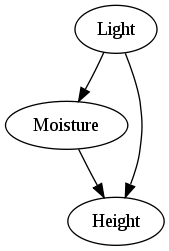
\includegraphics[scale=0.85]{PlantGrowth.png}
    \caption{Bayes Net considered within a plant growth study}
    \label{BNPlant}
  \end{center}
\end{figure}




It is necessary to adapt the Height discretization to the specific conditional distributions $(heightWhenDimAndWet$, $heightWhenBrightAndWet$, $heightWhenDimAndDry$, $heightWhenBrightAndDry$, thanks to the static method $AdaptGrid$ of the object $BayesNetAgrum$ proposed by the $otagrum$ python module.  The adaptation consists in adding, if necessary, some lower and upper bounds to the initial proposed grid so that all the probabilistic mass of  the conditional distributions be included in the final proposed grid. These lower and upper bounds are respectively the min and max of all the numerical lower and upper bounds of the conditional distributions. Furthermore, the initial grid may be potentially unsorted : the final grid is sorted.\\


This use case shows how to create such a variable : creation of the object and its modalities.\\

The corresponding lines are entirely part of the $pyagrum$ module, except for the adaptation of the global discretization which is only supported by the  $otagrum$ module.\\

 The quantification step is described further in section \ref{BayesNetQuantification}.\\

\requirements{
  \begin{description} 
  \item[$\bullet$] some conditional probability distributions : {\itshape dist1, dist2, dist3, dist4}
  \item[type:] Distribution, the $openturns$ object
  \end{description}
}
{
  \begin{description}
  \item[$\bullet$] a discretized variable  : {\itshape myDiscreteVar},
  \item[type:] a DiscretizedVar
  \end{description}
}



\espace

Python  script for this use case :

\begin{lstlisting}
# Create a Discretized variable

# Choose a name
name = 'MyName'
# Give a comment
comment = 'What I represent'
myDiscretizedVar = DiscretizedVar(name, comment)

###########################################################
# CASE 1 : The variable does not depend on other variables
###########################################################

# Give the suite of the interval bounds
# for example, the intervals are [0,1], [1, 3], [3, 10]
myDiscretizedVar.addTick(0)
myDiscretizedVar.addTick(1)
myDiscretizedVar.addTick(3)
myDiscretizedVar.addTick(10)



###################################################################
# CASE 2 : The variable depends on other variables
# Its conditional probability table depends on  4 conditional 
# distributions
# ==> You need to adapt the ticks to the conditional distributions
###################################################################

# Give a first proposition of bounds
# for example, initialData = (0,10,20, ..., 100)
initialTicks = NumericalPoint(range(0, 100, 10))

# Adapt the initial ticks to (dist1, dist2, dist3, dist4)
# Create a collection of distribution
finalTicks = BayesNetAgrum.AdaptGrid(
            DistributionCollection([dist1, dist2, dist3, dist4]), 
            initialTick)

# Set these new adapted ticks to the DiscretizedVar
for i in finalTicks : 
  myDiscretizedVar.addTick(i)

###########################################################

# Print the created discretized variable
print myDiscretizedVar

# Calculate the lenght of the range
lenght = len(myDiscretizedVar)

# Erase all the declared bounds
# the discretized variable has no range any more
myDiscretizedVar.eraseTicks()

# Test whether the real value is one of the range bounds suite
value = 3.4
print myDiscretizedVar.isTick(value)

# Explicitate the intervale [T_i, T_{i+1}]
i=2
print myDiscretizedVar.label(i)
\end{lstlisting}




%%%%%%%%%%%%%%%%%%%%%%%%%%%%%%%%%%%%%%%%%%%%%%%%%%%%%%%%%%%%%%
\newpage \subsection{Creation of a $pyagrum$ Bayes Net} \label{BayesNetCreation}



Once the variables have been created with their modalities as described in section \ref{VariableCreation}, the next step is to create a bayesian network through the $pyagrum$ module line commands, thanks to the object $BayesNet$. \\

It is important to note that the bayesian network object $BayesNet$ can be transformed into the bayesian network object $BayesNetAgrum$ proposed by $otagrum$ only once the $pyagrum$ object has been entirely quantified as described in section \ref{BayesNetQuantification}.\\

%%%%%%%%%%%%%%%%%%%%%%%%%%%%%%%%%%%%%%%%%%%%%%%%%%%%%%%%%%%%%%
\subsubsection{UC : Creation of the graph}

This use case shows how to create the graph of a bayesian network. It takes the example of the structure drawn in Fig.\ref{BNPlant}.\\

The corresponding lines are entirely part of the $pyagrum$ module. \\



\requirements{
  \begin{description} 
  \item[$\bullet$] some variables {\itshape moisture}, {\itshape light}, {\itshape height}
  \item[type:]  a LabelizedVar, a RangeVar or a Discretizedvar
  \end{description}
}
{
  \begin{description}
  \item[$\bullet$] a   $pyagrum$ bayesian network : {\itshape myBNpyagrum},
  \item[type:] a BayesNet
  \end{description}
}

\espace 
Python  script for this use case :

\begin{lstlisting}
# Create an empty bayesian network
netName = "Plant Growth"
myBNpyagrum = BayesNet(netName)

# Add variables to the bayesian network
indexLight    = myBNpyagrum.add(light)
indexMoisture = myBNpyagrum.add(moisture)
indexHeight   = myBNpyagrum.add(height)

# Create arcs
# Light -> Moisture
myBNpyagrum.insertArc(indexLight, indexMoisture)
#  Light -> Height
myBNpyagrum.insertArc(indexLight, indexHeight)
#  Moisture -> Height
myBNpyagrum.insertArc(indexMoisture, indexHeight)

# Print the created Bayes network
print myBNpyagrum

# Show the antecedents of moisture in the order in which they were created
print "moisture Antecedents= ", myBN.cpt(indexMoisture).var_names

# Erase a specific arc
# For example between Light and Moisture
myBNpyagrum.eraseArc(indexLight, indexMoisture)
\end{lstlisting}






%%%%%%%%%%%%%%%%%%%%%%%%%%%%%%%%%%%%%%%%%%%%%%%%%%%%%%%%%%%%%%
\newpage \subsection{Quantification of a Bayes Net} \label{BayesNetQuantification}


The quantification of a bayesian network consists in fulfilling the conditionnal probability table of each variable of the network. There are two different situations : 
\begin{itemize}
   \item the variable has no antecedent, and its probability table does not depend on the realization of other variables,
   \item the variable has at least one antecedent and its probability table is conditonned to the realization of its antecedent(s).
\end{itemize}


%%%%%%%%%%%%%%%%%%%%%%%%%%%%%%%%%%%%%%%%%%%%%%%%%%%%%%%%%%%%%%
\subsubsection{UC : Quantification of a Probability table }

This use case shows how to quantify the probability table of a variable which has no antecedent.\\

The corresponding lines are entirely part of the $pyagrum$ module. \\



\requirements{
  \begin{description} 
  \item[$\bullet$] a   $pyagrum$ bayesian network : {\itshape myBNpyagrum},
  \item[type:] a BayesNet
  \item[$\bullet$] one of its variable {\itshape light} with two modalities, 
  \item[type] a LabelizedVar, a RangeVar or a Discretizedvar
  \end{description}
}
{
  \begin{description}
  \item[$\bullet$] the quantified BayesNet : {\itshape myBNpyagrum},
  \item[type:] a BayesNet
  \end{description}
}

\espace 
Python  script for this use case :

\begin{lstlisting}
# Here we explicitate a line which has been declared previously
# at the creation step of myBNpyagrum
indexLight = myBNpyagrum.add(light)

# Fulfill the probability table
# Modalities are sorted in the order where they were created
# for example, Proba(light== first modality) = 0.25
# for example, Proba(light== second modality) = 0.75
myBNpyagrum.cpt(indexLight)[:]= [0.25, 0.75]
\end{lstlisting}


%%%%%%%%%%%%%%%%%%%%%%%%%%%%%%%%%%%%%%%%%%%%%%%%%%%%%%%%%%%%%%
\newpage \subsubsection{UC : Quantification of a Conditional Probability table }

This use case shows how to quantify the conditional probability table  of a variable which has at least one antecedent.\\

Several cases are treated : 
\begin{itemize}
  \item the variable is a LabelizedVar (or a RangeVar),
  \item the variable is a DiscretizedVar.
\end{itemize}


The corresponding lines are  part of the $pyagrum$ module in the fisrt case.  The second case requires the use of $otagrum$ which proposes the method $BayesNetAgrum.Discretize$ to discretize a continuous distribution of $openturns$ in order to fulfill the conditional probability table of the $pyagrum$ variable.\\

This use case illustrates the example of Fig.\ref{BNPlant}. We suppose the conditionnal probability table described in Tab.\ref{condTP2}.\\

\begin{table}[H]
  \begin{center}
    \begin{tabular}{c|c|c}
      $Moisture$ - $Light$ & $Dim$ & $Bright$ \\
      \hline
      $Wet$ & heightWhenDimAndWet &  heightWhenBrightAndWet\\
      \hline
      $Dry$ & heightWhenDimAndDry &  heightWhenBrightAndDry
    \end{tabular}
    \caption{Example of a conditional table of probability.}
    \label{condTP2}
  \end{center}
\end{table}


\requirements{
  \begin{description} 
  \item[$\bullet$] a   $pyagrum$ bayesian network : {\itshape myBNpyagrum},
  \item[type:] a BayesNet
  \item[$\bullet$] its variables {\itshape light} and {\itshape moisture}  
  \item[type] a LabelizedVar 
  \item[$\bullet$] its variable {\itshape height} 
  \item[type] a DiscretizedVar
  \item[$\bullet$] some  distributions {\itshape heightWhenDimAndWet, ...} 
  \item[type] some $openturns$ Distribution
  \end{description}
}
{
  \begin{description}
  \item[$\bullet$] the quantified BayesNet : {\itshape myBNpyagrum},
  \item[type:] a BayesNet
  \end{description}
}

\espace 
Python  script for this use case :

\begin{lstlisting}
# Here we explicitate some lines which have been declared previously
# at the creation step of myBNpyagrum
indexMoisture = myBNpyagrum.add(moisture)
indexHeight = myBNpyagrum.add(height)

# We show the antecedents of these variables with the order in which they were created
print "Moisture Antecedents= ", myBNpyagrum.cpt(indexMoisture).var_names
print "Height Antecedents= ", myBNpyagrum.cpt(indexHeight).var_names




######################################################################
# CASE 1 : The  LabelizedVar (or RangeVar) depends on a Labelized one
######################################################################
# Fulfill the probability table when light='Dim'
# we recall that the name of light is Light
myBNpyagrum.cpt(indexMoisture)[{'Light' : 'Dim'}] = [0.2, 0.8]

# Fulfill the probability table when light='Bright'
myBNpyagrum.cpt(indexMoisture)[{'Light' : 'Bright'}] = [0.6, 0.4]


######################################################################
# CASE 2 : The  LabelizedVar (or RangeVar)  depends on a RangeVar 
######################################################################
# Fulfill the  probability table when myRangeVar= its first modality (it means 3)
myBNpyagrum.cpt(indexMoisture)[{'nameRange' : 0}]= [0.2, 0.8]

# Fulfill the  probability table when myRangeVar= its second modality (it means 4)
myBNpyagrum.cpt(indexMoisture)[{'nameRange' : 1}]= [0.2, 0.8]

# Fulfill the  probability table when myRangeVar= its third modality (it means 5)
myBNpyagrum.cpt(indexMoisture)[{'nameRange' : 2}]= [0.2, 0.8]


########################################################################
# CASE 3 : The  Discretized one  depends on a LabelizedVar (or RangeVar)
########################################################################
# We have to enter some openturns distributions 
# within pyagrum conditional probability tables

# We suppose that the discretization data has been 
# adapted to the conditional distributions

# The new class BayesNetAgrum from otagrum is able to marry OT distributions 
# and pyagrum conditional probability tables
myBN.cpt(indexHeight)[{'Light': 'Dim', 'Moisture': 'Dry'}]   = ...
                       ... BayesNetAgrum.Discretize(heightWhenDimAndDry, data)
myBN.cpt(indexHeight)[{'Light': 'Bright', 'Moisture': 'Dry'}] =  ...
                       ... BayesNetAgrum.Discretize(heightWhenBrightAndDry, data)
myBN.cpt(indexHeight)[{'Light': 'Dim', 'Moisture': 'Wet'}]    = ...
                       ...  BayesNetAgrum.Discretize(heightWhenDimAndWet, data)
myBN.cpt(indexHeight)[{'Light': 'Bright', 'Moisture': 'Wet'}] =  ...
                       ... BayesNetAgrum.Discretize(heightWhenBrightAndWet, data)
\end{lstlisting}



%%%%%%%%%%%%%%%%%%%%%%%%%%%%%%%%%%%%%%%%%%%%%%%%%%%%%%%%%%%%%%
\newpage \subsection{Propagation of Uncertainty within a bayesian network} \label{BayesNetPropagation}

This section explicitates how to propagate uncertainties through a bayesian network. The $otagrum$ helps to link the $pyagrum$ bayesian network to the $openturns$ functionalities. The first step is then to transform a $pyagrum$ bayesian network into a $otagrum$ one. Then, it is possible to extract the distribution of some variables and to manipulate them thanks to the $openturns$ functionalities, as described in the Openn TURNS Use Cases Guide.




%%%%%%%%%%%%%%%%%%%%%%%%%%%%%%%%%%%%%%%%%%%%%%%%%%%%%%%%%%%%%%
\subsubsection{UC : Creation of the $otagrum$ Bayes Net from the $pyagrum$ Bayes Net}

It is important to note that the bayesian network object $BayesNet$ can be transformed into the bayesian network object $BayesNetAgrum$ proposed by $otagrum$ only once the $pyagrum$ object has been entirely quantified as described in section \ref{BayesNetQuantification}.\\
This transformation enables to use the $otagrum$ functionalities which links the $pyagrum$ bayesian network to the $openturns$ functionalities.\\


\requirements{
  \begin{description} 
  \item[$\bullet$] a  quantified  $pyagrum$ bayesian network : {\itshape myBNpyagrum},
  \item[type:] a BayesNet
  \end{description}
}
{
  \begin{description}
  \item[$\bullet$] the $openturns$ bayesian network : {\itshape myBNot},
  \item[type:] a BayesNetAgrum
  \end{description}
}

\espace 

Python  script for this use case :

\begin{lstlisting}
# Create a BayesNetAgrum object
myNBot = BayesNetAgrum(myBNpyagrum)
\end{lstlisting}


%%%%%%%%%%%%%%%%%%%%%%%%%%%%%%%%%%%%%%%%%%%%%%%%%%%%%%%%%%%%%%
\newpage \subsubsection{UC : Bayesian inference through the  $openturns$ Bayes Net}

This use case shows how to manipulate a $otagrum$ bayesian network, in particular how to : 
\begin{itemize}
  \item set an evidence, which means give a particular value to a variable of the network, thanks to the method {\itshape setEvidence}, and the reverse action {\itshape eraseEvidences},
  \item get the marginal distribution of a variable thanks to the method {\itshape getMarginal}.
\end{itemize}

The corresponding lines are  proposed by the $otagrum$ module.\\

For example, this use case studies the  situation drawn in Fig.\ref{BNPlant}.\\

\requirements{
  \begin{description} 
  \item[$\bullet$] the $openturns$ bayesian network : {\itshape myBNot}
  \item[type:] a BayesNetAgrume
  \item[$\bullet$] its variable {\itshape light} 
  \item[type] a LabelizedVar which name is 'Light' and one of its modality 'Bright'
  \item[$\bullet$] its variable {\itshape height} 
  \item[type] a DiscretizedVar which name is 'Height'
  \item[$\bullet$] its variable {\itshape myRangeVar} (added to the example)
  \item[type] a RangeVar which name is 'MyRangeVar' and one of its modality 3
  \end{description} 
}
{
  \begin{description}
  \item[$\bullet$] the marginal distribution of of {\itshape light} and {\itshape height} 
  \item[type:]  Distribution, objects of $openturns$
  \end{description}
}

\espace 

Python  script for this use case :

\begin{lstlisting}
# Get the distribution of a the variable 'Height'
heightDistribution = myBNot.getMarginal("Height")

# This marginal distribution is a Distribution object of openturns
# Manipulate it as decsribed in the Open TURNS Use Cases Guide

# Set the 'Light' LabelizedVar variable to its modality 'Bright'
otbn.setEvidence("Light", "Bright")

# Set the 'MyRangeVar' RangeVar variable to its modality 3
# where myRangeVar = RangeVar('MyRangeVar', 'comment',3,5)
otbn.setEvidence("'MyRangeVar'", 3)

# Set the 'Height' DiscretizedVar variable to its modality 
# containing the real 1.2
otbn.setEvidence("Height", 1.2)

# Erase all the set evidences of the bayesian network
otbn.eraseEvidences()
\end{lstlisting}


%%%%%%%%%%%%%%%%%%%%%%%%%%%%%%%%%%%%%%%%%%%%%%%%%%%%%%%%%%%%%%%%%%%%
\newpage \subsubsection{UC : Save and Load a  $otagrum$  Bayes Net through a BIF  format file}


This use case shows how to save a $otagrum$  bayesian network into a BIF format file and how to load a $otagrum$ bayesian network from a such a file. \\

It is important to note that the BIF format file created from the $otagrum$  bayesian network is not compatible with the BIF format since it uses some forbidden graphic signs as '[', ']', ';', '(' and ')'. It comes from the fact that the BIF format is not compatible with the  variables of type $DiscretizedVar$ : consequently, these variables are  saved under $LabelizedVar$, which labels require the use of the forbidden graphic signs.\\
Then, the BIF format file producted here can  be reload by the $otagrum$ functionality presented in this use case only which corrects the forbidden graphic signs. Be careful : as explained previously, the $DiscretizedVar$ is reload under the type $LabelizedVar$ wich changes its manipulation.\\

The BIF format file producted, even if not theoritically correct, is nevertheless interesting because easily understandable but the Reader.\\

\requirements{
  \begin{description} 
  \item[$\bullet$] the $openturns$ bayesian network : {\itshape myBNot},
  \item[type:] a BayesNetAgrum
  \item[$\bullet$] a BIF format file containing a $otagrum$ bayesian network : {\itshape myBN\_BIF\_file.bif },
  \item[type:] a BIF format file obtained by the $otagrum$ save functionality
  \end{description}
}
{
  \begin{description}
  \item[$\bullet$] the $openturns$ bayesian network load from the BIT format file: {\itshape myReloadBNot},
  \item[type:] a BayesNetAgrum
  \end{description}
}

\espace 

Python  script for this use case :

\begin{lstlisting}
#########################################################
# Case 1 : Export a bayesian network in a BIF format file
#########################################################
# Care : mention the BIF extension
netName = myOTBayesNet
myBNot.exportToBIFFile(netName+".bif")

#########################################################
# Case 2 : Load a bayesian network from a BIF format file
#########################################################
myReloadBNot=BayesNetAgrum('myBN_BIF_file.bif')
\end{lstlisting}



%%%%%%%%%%%%%%%%%%%%%%%%%%%%%%%%%%%%%%%%%%%%%%%%%%%%%%%%%%%%%%%%%%%%
\newpage \subsubsection{UC : Graphic and text vizualisation  of the $otagrum$  Bayes Net}


This use case shows how to vizualize a $otagrum$ bayesian network either :
\begin{itemize}
  \item under a text sum up of the network, thanks to the method {\itshape print},
  \item with a graphic, thanks to the method {\itshape draw}.
\end{itemize}
Furthermore, the $BayesNetAgrum$ object may be stored through a StorageManager according to the mecanism proposed by $openturns$ : see the Open TURNS Use Cases Guide to have the description of this mecanism.\\


\requirements{
  \begin{description} 
  \item[$\bullet$] the $openturns$ bayesian network : {\itshape myBNot},
  \item[type:] a BayesNetAgrum
  \end{description}
}
{
  \begin{description}
  \item[$\bullet$] a graphic of the network, 
  \item[type:] a PNG format fiel
  \end{description}
}

\espace 

Python  script for this use case :

\begin{lstlisting}
# Draw the network structure within a PNG format file
myBNot.draw('myBNGraph')

# Give the text sum up of the network
print myBNot
\end{lstlisting}